\documentclass{scrartcl}

\usepackage{graphicx}
\usepackage[utf8]{inputenc}
\usepackage[T1]{fontenc}
\usepackage{lmodern}
\usepackage[english]{babel}
\usepackage{amsmath}
\usepackage{amsthm}
\usepackage{mathtools}
\usepackage{amssymb}
\usepackage{listings}
\usepackage{xparse}
\usepackage{geometry}
\usepackage{enumerate}
\usepackage{tikz}
\usepackage{hyperref}
\usepackage[style=english]{csquotes}
\usepackage[language=english, backend=biber, style=alphabetic, sorting=nyt]{biblatex}

\hypersetup{
    colorlinks,
    linkcolor={red!50!black},
    citecolor={blue!50!black},
    urlcolor={blue!80!black}
}

\usetikzlibrary{babel, positioning, shapes.geometric, arrows, arrows.meta}
\addbibresource{bibliography.bib}

\title{Miniproject - Introduction to Schemes}
\author{Candidate Number: 1059926}

\newcommand{\N}{\mathbb{N}}
\newcommand{\Z}{\mathbb{Z}}
\newcommand{\F}{\mathbb{F}}
\newcommand{\C}{\mathbb{C}}
\newcommand{\Q}{\mathbb{Q}}
\newcommand{\V}[1]{\mathrm{V}_+(#1)}
\newcommand{\D}[1]{\mathrm{D}_+(#1)}
\newcommand{\A}{\mathbb{A}}
\renewcommand{\P}{\mathbb{P}}
\newcommand{\p}{\mathfrak{p}}
\newcommand{\q}{\mathfrak{q}}
\newcommand{\m}{\mathfrak{m}}
\renewcommand{\a}{\mathfrak{a}}
\renewcommand{\b}{\mathfrak{b}}
\renewcommand{\m}{\mathfrak{m}}
\newcommand{\Nil}{\mathfrak{N}}
\newcommand{\Set}{\mathrm{\textbf{Set}}}
\newcommand{\Aff}{\mathrm{\textbf{Aff}}}
\newcommand{\Sch}{\mathrm{\textbf{Sch}}}
\newcommand{\Ring}{\mathrm{\textbf{Ring}}}
\newcommand{\Ab}{\mathrm{\textbf{Ab}}}
\newcommand{\Top}{\mathrm{Top}}
\newcommand{\Spec}{\mathrm{Spec}}
\newcommand{\Proj}{\mathrm{Proj}}
\newcommand{\Frac}{\mathrm{Frac}}
\newcommand{\im}{\mathrm{im}}
\newcommand{\cont}{\mathrm{cont}}
\renewcommand{\O}{\mathcal{O}}
\DeclareMathOperator*{\colim}{colim}
\newcommand{\citestacks}[1]{\cite[\href{https://stacks.math.columbia.edu/tag/#1}{Tag #1}]{stacks}}

\newcommand\restr[2]{{
    \left.\kern-\nulldelimiterspace
    #1
    \vphantom{\big|}
    \right|_{#2}
}}

\newtheorem{prop}[subsection]{Proposition}
\newtheorem{theorem}[subsection]{Theorem}
\newtheorem{lemma}[subsection]{Lemma}
\newtheorem{corollary}[subsection]{Corollary}

\theoremstyle{definition}
\newtheorem{problem}[subsection]{Problem}
\newtheorem{alg}[subsection]{Algorithm}
\newtheorem{definition}[subsection]{Definition}
\newtheorem{example}[subsection]{Example}
\newtheorem{remark}[subsection]{Remark}
\newtheorem{reminder}[subsection]{Reminder}

\begin{document}
\maketitle

\tableofcontents

\section{Definition of $\Proj$}

First of all, we introduce the fundamental object used in the $\Proj$-construction.
\begin{definition}
    A \emph{graded ring}\footnote{
        Unlike most authors, we consider graded rings with homogeneous elements of negative degree (i.e. not naturally graded rings), so that we can talk about the grading of a localization.
        Namely, if $T \subseteq S$ is a multiplicative subset containing only homogeneous elements of a graded ring $S$, then $T^{-1}S$ has the canonical grading given by $\deg(f/t) = \deg(f) - \deg(t)$.
    } $S$ is a ring $S$ with a decomposition $S = \oplus_{d \in \Z} S_d$ into subgroups $S_i \subseteq S$ (w.r.t. addition in $S$) such that $S_i \cdot S_j \subseteq S_{i + j}$ for all $i, j \in \Z$.
    We call $S$ \emph{naturally graded}, if $S_i = \{ 0 \}$ for $i < 0$.
    Write further $S_+ := \sum_{d \neq 0} S_d$.
    For a homogeneous $f \in S_d$ say that $\deg(f) := d$ is its \emph{degree}.

    An element $f \in S$ is called \emph{homogeneous} (of degree $n$), if $f \in S_n$.
    An ideal $I \leq S$ is called \emph{homogeneous}, if it has a set of homogeneous generators.
\end{definition}
From now on let $S$ be a naturally graded ring.
\begin{definition}
    Define the \emph{projective spectrum} $\Proj(S)$ as all homogeneous prime ideals that do not contain the ``irrelevant ideal'' $S_+$
    \begin{equation*}
        \Proj(S) := \{ \p \in \Spec(S) \ | \ \text{$\p$ homogeneous}, \ S_+ \not\subseteq \p \}
    \end{equation*}
    This becomes a topological space by endowing it with the \emph{Zariski-topology} on $\Proj(S)$, given by the open sets
    \begin{equation*}
        \D{\a} := \{ \p \in \Proj(S) \ | \ \a \not\subseteq \p \}
    \end{equation*}
    for any homogeneous ideal $\a \leq S$.
\end{definition}
\begin{prop}
    The above definition is well-defined, i.e. the sets $\D{\a}$ indeed form a topology on $\Proj(S)$.
\end{prop}
\begin{proof}
    Clearly $\Proj(S) = \D{\langle 1 \rangle}$ and $\emptyset = \D{\langle 0 \rangle}$ are open.
    To show that finite intersections and arbitrary unions of open sets are open, notice that as usual
    \begin{equation*}
        \D{\a} \cap \D{\b} = \D{\a\b} \quad \text{and} \quad \bigcup_{\a \in \mathcal{A}} \D{\a} = \D{\b} \quad \text{where} \ \b = \sum_{\a \in \mathcal{A}} \a
    \end{equation*}
    Clearly the ideals $\a\b$ and $\b$ are again homogeneous.
\end{proof}
As opposed to Hartshorne \cite{hartshorne}, our approach to construct a sheaf of rings on $\Proj(S)$ will be similar to the construction of $\Spec(R)$, i.e. we will first specify $\O_{\Proj(S)}$ on a topological basis.
This is also the definition used in \citestacks{01M6}.
\begin{lemma}
    \label{prop:Splus_invariance}
    For a homogeneous ideal $\a$ have $\D{\a} = \D{\a S_+}$.
\end{lemma}
\begin{proof}
    The inclusion $\supseteq$ is clear, as $\a S_+ \subseteq \a$.
    So assume there is a $\p \in \D{\a}$.
    Since $\p \in \Proj(S)$ find $S_+ \not\subseteq \p$ and by assumption, $\a \not\subseteq \p$.
    Thus there are $s \in S_+$ and $a \in \a$ with $a, s \notin \p$.
    Since $\p$ is prime, it follows that $as \notin \p$ and so $\a S_+ \not\subseteq \p$.
\end{proof}
\begin{prop}
    \label{prop:basis_topology}
    The sets $\D{f} := \D{\langle f \rangle}$ for homogeneous $f \in S_+$ form a basis of the topology on $\Proj(S)$.
\end{prop}
\begin{proof}
    Clearly $\langle f \rangle$ is a homogenous ideal, so $\D{f}$ is open.
    For any homogeneous ideal $\a = \langle f_i \ | \ i \in I \rangle$ with $f_i \in S$ homogeneous have that $\D{\a} = \D{\a S_+}$ by Lemma~\ref{prop:Splus_invariance}, so we can assume wlog that all $f_i \in S_+$.
    Now have
    \begin{equation*}
        \D{\a} = \bigcup_{i \in I} \D{f_i}
    \end{equation*}
    as $\a \not\subseteq \p$ implies there is some $g = \sum_{i \in I} g_i f_i \notin \p$, with $g_i \in S$.
    Hence, at least one $g_j f_j \notin \p$ and so $f_j \notin \p$, thus $\p \in \D{f_j}$.
    It follows that the $\D{f}$ generate the topology on $\Proj(S)$, so it is left to show that they are a basis.

    Consider $\p \in \D{f} \cap \D{g}$, so $f, g \notin \p$.
    Since $\p$ is prime, it follows that $fg \notin \p$ and so $\D{fg} \subseteq \D{f} \cap \D{g}$ is an open neighborhood of $\p$.
\end{proof}
\begin{lemma}
    \label{prop:homogeneous_part_prime}
    Let $\p \leq S$ be a prime ideal.
    Then
    \begin{equation*}
        \p' := \langle f \in \p \ | \ \text{$f$ homogeneous} \rangle \leq S
    \end{equation*}
    is a (homogeneous) prime ideal.
\end{lemma}
\begin{proof}
    Consider $f, g \in S$ with $f g \in \p'$ and assume $f, g \notin \p'$.
    Write $f = \sum_d f_d$ and $g = \sum_d g_d$ with $f_d, g_d \in S_d$.
    So
    \begin{equation*}
        \sum_{i, j} f_i g_j = \sum_n \sum_{i + j = n} f_i g_j \in \p'
    \end{equation*}
    Since $\p'$ is homogeneous, it follows that
    \begin{equation*}
        \sum_{i + j = n} f_i g_j \in \p'
    \end{equation*}
    for all $n \in \Z$.
    Let now $d$ resp. $e$ be maximal such that $f_d \notin \p'$ resp. $g_e \notin \p'$.
    We have
    \begin{equation*}
        f_d g_e + \sum_{\substack{i + j = d + e\\(i, j) \neq (d, e)}} \underbrace{f_i g_j}_{\in \p'} = \sum_{i + j = d + e} f_i g_j \in \p'
    \end{equation*}
    and so $f_d g_e \in \p' \subseteq \p$.
    Since $\p$ is prime, it follows that $f_d \in \p$ or $g_e \in \p$.
    However both $f_d$ and $g_e$ are homogeneous, so $f_d \in \p'$ or $g_e \in \p'$, a contradiction.
\end{proof}
\begin{lemma}[``Covering Trick'']
    \label{prop:covering_trick}
    Let $f, f_i \in S_+$ be homogeneous.
    Then $\D{f} \subseteq \bigcup_i \D{f_i}$ if and only if $f^n \in \langle f_i \ | \ i \rangle$ for some $n \in \N$
\end{lemma}
\begin{proof}
    The direction $\Leftarrow$ is clear.
    So assume $\D{f} \subseteq \bigcup_i \D{f_i}$.
    If no $f^n$ is in $\a := \langle f_i \ | \ i \rangle$, then $f$ is not nilpotent in $S/\a$ and so $(S/\a)_f$ is not the zero ring.
    Hence, $(S/\a)_f$ has a prime ideal, and its preimage under $S \to S/\a \to (S/\a)_f$ yields a prime ideal $\p'$ containing $\a$ and not containing $f$.
    Since $f \in S_+$ note that $S_+ \not\subseteq \p'$ and as both $f$ and $\a$ are homogeneous, Lemma~\ref{prop:homogeneous_part_prime} yields now that $\langle g \in \p' \ | \ \text{$g$ homogeneous} \rangle$ is a prime ideal in $\D{f}$ but not in $\bigcup_i \D{f_i}$, contradicting the assumption.
\end{proof}
\begin{corollary}
    \label{prop:basic_set_inclusion_divisibility}
    If $\D{g} \subseteq \D{f}$ with $f, g \in S_+$, then there is a homogeneous $h \in S$ such that $g^n = fh$ for some $n \in \N$.
\end{corollary}
\begin{proof}
    By assumption, $\D{f}$ covers $\D{g}$, thus by the Covering Trick (Lemma~\ref{prop:covering_trick}), observe that $g^n \in \langle f \rangle$ for some $n \in \N$.
    The claim follows.
\end{proof}
\begin{prop}
    Let $B = \{ \D{f} \ | \ \text{$f \in S_+$ homogeneous}\}$.
    The functor\footnote{The map on arrows is well-defined by Corollary~\ref{prop:basic_set_inclusion_divisibility}.}
    \begin{align*}
        \mathcal{F}: \restr{\Top(\Proj(S))}{B} \to \Ring, \quad \D{f} &\mapsto (S_f)_0 \\
        (\D{fg} \subseteq \D{f}) &\mapsto \Bigl( \restr{\cdot}{\D{fg}}: \frac s {f^n} \mapsto \frac {sg^n} {(fg)^n} \Bigr)
    \end{align*}
    is a B-sheaf on $B$ (here $\Top(X)$ is the category given by the open sets of $X$ and their inclusion, as defined in the lecture).
\end{prop}
\begin{proof}\footnote{I guess I have included the proof mostly for the sake of completeness - apart from presentational issues, it is just copied from the lecture notes.}
    Clearly, $\mathcal{F}$ is a functor and thus a presheaf.
    Hence, we have to show the local-to-global property.

    Let $\D{f} = \bigcup_{i \in I} \D{g_if}$ be a cover and $s_i \in \mathcal{F}(\D{g_if})$ such that
    \begin{equation*}
        \forall x \in \D{g_if} \cap \D{g_jf} \ \exists V \in B: \ V \subseteq \D{g_if} \cap \D{g_jf}, \ x \in V, \ \frac {s_i} 1 = \frac {s_j} 1 \in \mathcal{F}(V)
    \end{equation*}
    We show that the $s_i$ glue to a unique $s \in \mathcal{F}(\D{f})$.
    To show uniqueness, assume there are $\alpha/f^N, \beta/f^N \in \D{f}$ with
    \begin{equation*}
        \restr{\frac {\alpha} {f^N}}{\D{g_if}} = \restr{\frac {\beta} {f^N}}{\D{g_if}} \quad \text{for all $i$}
    \end{equation*}
    Therefore there is $n_i \in \N$ such that
    \begin{equation*}
        (f g_i)^{n_i} (\alpha f^N + \beta f^N) = 0
    \end{equation*}

    wlog there are only finitely many $i$ (by the Covering Trick, Lemma~\ref{prop:covering_trick}).

    wlog $N$ is sufficiently large (we can always increase $N$), and so $(fg_i)^N(\alpha - \beta) = 0$.

    Since $\bigcup_i \D{(fg_i)^N} = \bigcup_i \D{fg_i} = \D{f}$ it follows that $f^n \in \langle (fg_i)^N \ | \ i \rangle$ for some $n \in \N$ (again the Covering Trick, Lemma~\ref{prop:covering_trick}).
    Therefore we find
    \begin{equation*}
        f^n(\alpha - \beta) \in \langle (f g_i)^N \ | \ i \rangle (\alpha - \beta) = \langle (f g_i)^N (\alpha - \beta) \ | \ i \rangle = \{ 0 \}
    \end{equation*}
    and so $\alpha = \beta \in S_f$.

    Now we show existence.
    By the uniqueness above, it follows that
    \begin{equation*}
        \restr{s_i}{\D{fg_ig_j}} = \restr{s_i}{\D{fg_i} \cap \D{fg_j}} = \restr{s_j}{\D{fg_i} \cap \D{fg_j}} = \restr{s_j}{\D{fg_ig_j}}
    \end{equation*}
    wlog have again a finite cover, i.e. only finitely many $g_i$.
    Hence find an $N \in \N$ such that each $s_i = s'_i / (fg_i)^N$ with $s'_i \in S$ homogeneous.
    By possibly replacing $N$ with a bigger $N$, we can now assume that
    \begin{equation*}
        (f^2g_ig_j)^N \left( s'_i (f g_j)^N - s'_j (f g_i)^N \right) = 0 \quad \text{as $\restr{s_i}{\D{fg_ig_j}} = \restr{s_j}{\D{fg_ig_j}}$}
    \end{equation*}
    Now note that
    \begin{equation*}
        s_i = \frac {a_i} {b_i} \quad \text{with}\ a_i = s'_i(f g_i)^N, \ b_i = (f g_i)^{2N}
    \end{equation*}
    and
    \begin{equation*}
        a_i b_j - a_j b_i = s'_i (f g_i)^N (f g_j)^{2N} - s'_j (f g_j)^N (f g_i)^{2N} = \underbrace{(f^2g_ig_j)^N \left(s'_i (fg_j)^N - s'_j (fg_i)^N \right)}_{= 0}
    \end{equation*}
    Now observe that $\D{b_i} = \D{fg_i}$ and so $f^n \in \langle b_i \ | \ i \rangle$ for some $n$ (once again the Covering Trick, Lemma~\ref{prop:covering_trick}).
    Let $f^n = \sum_i r_i b_i$ and get
    \begin{equation*}
        a_i f^n = \sum_l r_l b_l a_i = \sum_l r_l a_l b_i = b_i \sum_l r_l a_l
    \end{equation*}
    Note that $a_i, b_i, f$ are homogeneous, and so we can also choose $r_i$ to be homogeneous.
    Then find that $0 = \deg(s_i) = \deg(a_i) - \deg(b_i) = \deg(\sum r_l a_l) - n\deg(f)$.

    Thus
    \begin{equation*}
        s_i = s := \frac {\sum_l r_l a_l} {f^n} \in S_f
    \end{equation*}
    and since $\deg(\sum r_l a_l) = n\deg(f)$ we find that $s \in (S_f)_0 = \mathcal{F}(\D{f})$.
    Clearly $\restr{s}{\D{fg_i}} = s_i$ and the claim follows.
\end{proof}
Now the B-sheaf extension theorem from the lecture (from Section 1.11) yields the following corollary.
\begin{corollary}
    The B-sheaf $\mathcal{F}$ can be (uniquely, up to isomorphism) extended to a sheaf $\O_{\Proj(S)}$ on $\Proj(S)$.
\end{corollary}
The next to lemmas are based on \cite[Prop. II.2.5]{hartshorne} and will be used to deduce that $(\Proj(S), \O_{\Proj(S)})$ is a scheme.
\begin{lemma}
    For $\p \in \Proj(S)$, the stalk
    \begin{equation*}
        \O_{\Proj(S), \p} = (T^{-1}S)_0
    \end{equation*}
    is a local ring, where $T = \{ f \notin \p \ | \ \text{$f$ homogeneous}\}$ contains all homogeneous elements not in $\p$.
\end{lemma}
\begin{proof}
    Consider the ideal
    \begin{equation*}
        \m = \Bigl\{ \frac f g \in (T^{-1}S)_0 \ \Bigm| \ f \in \p \Bigr\}
    \end{equation*}
    We claim this is the unique maximal ideal of $(T^{-1}S)_0$.

    First, note that $1 \notin \m$ as otherwise, there would be $f/g \in T^{-1}S, f \in \p$ with $t(f - g) = 0$ for some $t \in T$.
    However then $tg = tf \in \p$, and so $g \in \p$ (as $t \notin \p$), contradicting $g \in T$.
    
    Now consider an ideal $\a$ such that $\a \setminus \m \neq \emptyset$, i.e. there is $f/g \in \a \setminus \m$.
    Then $f \in T$ as $f$ homogeneous (since $f/g \in (T^{-1}S)_0$ is homogeneous of degree 0) and $f \notin \p$.
    Thus $g/f \in (T^{-1}S)_0$ and so $f/g \in (T^{-1}S)_0^*$, which implies $\a = \langle 1 \rangle$.
\end{proof}
\begin{lemma}
    \label{prop:Df_affine}
    For $f \in S_+$ homogeneous have that $(\D{f}, \restr{\O_{\Proj(S)}}{\D{f}})$ is an affine scheme.
\end{lemma}
\begin{proof}
    Let $R = (S_f)_0$.
    Consider the map
    \begin{equation*}
        \phi: \D{f} \to \Spec(R), \quad \p \mapsto \p S_f \cap R
    \end{equation*}
    Note that it is continuous, as the preimage of some basic open set $D_{g/f^n}$ is $\D{fg} \subseteq \D{f}$ open.
    Furthermore, have the map
    \begin{equation*}
        \phi': \Spec(R) \to \D{f}, \quad \p \mapsto \p S_f \cap S
    \end{equation*}
    which is also continuous, as the preimage of some basic open set $\D{fg}$ is $D_{g^n/f^m}$ where $n\deg(g) = m\deg(f), (n, m) \neq (0, 0)$.
    Note that $\phi \circ \phi' = \mathrm{id}_{\Spec(R)}$ because for $\p \leq R$ have $\p \subseteq (\p S_f \cap S) S_f \cap R$ and
    \begin{equation*}
        (\p S_f \cap S) S_f \cap R \subseteq \p S_f \cap S_f \cap R = \p S_f \cap (S_f)_0 = \p
    \end{equation*}
    where the last equality holds, since $\p \leq (S_f)_0$ is homogeneous.
    
    To see that $\phi' \circ \phi = \mathrm{id}_{\D{f}}$, it suffices now to show that $\phi$ is injective ($\phi$ has a right-inverse, hence it is then bijective, and the one-sided inverse $\phi'$ is already the inverse).
    Let $\p, \q \leq S$ homogeneous primes with $f \notin \p, \q$.
    Assume there is $g \in \p \setminus \q$.
    Then
    \begin{equation*}
        g^{\deg(f)} \in \p S_f \setminus \q S_f  \ \Rightarrow \ \frac {g^{\deg(f)}} {f^{\deg(g)}} \in (\p S_f \setminus \q S_f) \cap R = (\p S_f \cap R) \setminus (\q S_f \cap R)
    \end{equation*}
    and so $\phi(\p) \neq \phi(\q)$. Thus $\phi$ is a homeomorphism.

    Now consider the natural transformation
    \begin{equation*}
        \eta: \O_{\Spec R} \Rightarrow \phi_*\Bigl( \restr{\O_{\Proj(S)}}{\D{f}} \Bigr)
    \end{equation*}
    given on basic open sets by
    \begin{equation*}
        \eta_{D_{g/f^n}}: R_{g/f^n} \to (S_{f g})_0, \quad \frac {h/f^m} {(g/f^n)^l} \mapsto \frac {h f^{nl}} {g^l f^m}
    \end{equation*}
    Clearly this is a ring isomorphism, so $\eta$ is a natural isomorphism.
    The claim follows.
\end{proof}
\begin{corollary}
    $(\Proj(S), \O_{\Proj(S)})$ is a scheme.
\end{corollary}

\section{Projective space}
For this section, let $R$ be a ring and assume $S$ is a graded $R$-algebra, i.e. $S$ is a graded ring with $R \subseteq S_0$.
\begin{definition}
    The scheme $\Proj(S)$ naturally becomes a scheme over $\Spec(R)$ via
    \begin{align*}
        &f: \Proj(S) \to \Spec(R), \quad \p \mapsto \p \cap R \\
        &f^\#_{D_f}: R_f \to \O_{\Proj(S)}(\D{f}) = (S_f)_0, \quad r \mapsto r
    \end{align*}
    This is well-defined, as $R \subseteq S_0$ implies $R_f \subseteq (S_0)_f = (S_f)_0$ since $\deg(f) = 0$.
\end{definition}
\begin{prop}
    \label{prop:projective_space_separated}
    The morphism $\Proj(S) \to \Spec(R)$ is separated.
\end{prop}
\begin{proof}
    This is the same proof as for \citestacks{01MC}.
    By Lemma~\ref{prop:Df_affine} we find a cover $\Proj(S) = \bigcup_i \D{f_i}$ of affine opens.
    We use the characterization from the lecture and show that $\D{f_i} \cap \D{f_j}$ is an affine open and the canonical multiplication map
    \begin{equation*}
        \O_{\Proj(S)}(\D{f_i}) \times \O_{\Proj(S)}(\D{f_j}) \to \O_{\Proj(S)}(\D{f_i} \cap \D{f_j})
    \end{equation*}
    is surjective.
    
    First note that $\D{f_i} \cap \D{f_j} = \D{f_if_j}$ which is affine open by Lemma~\ref{prop:Df_affine}.
    By definition, we have $\O_{\Proj(S)}(\D{f}) = (S)_0$ and so we have to show that
    \begin{equation*}
        (S_{f_i})_0 \times (S_{f_j})_0 \to (S_{f_if_j})_0, \quad (a, b) \mapsto ab
    \end{equation*}
    is surjective.

    For $g/(f_if_j)^n \in (S_{f_if_j})_0$ we now have that
    \begin{equation*}
        \frac {gf_j^r} {f_i^{n + t}} \cdot \frac {f_i^t} {f_j^{n + r}} = \frac g {(f_if_j)^n}
    \end{equation*}
    where $r, t \in \N$ such that\footnote{This exists, since $\gcd(\deg(f_i), \deg(f_j)) \ \mid \ \deg(f_j) \ | \ \deg(f_j)n$.} $\deg(f_j) n = \deg(f_i) t - \deg(f_j) r$.

    Since $\deg(g) = (\deg(f_i) + \deg(f_j)) n$ it follows that $\deg(g) + \deg(f_j)r = \deg(f_i) (n + t)$ and so both $gf_j^r/g_i^{n + t}$ and $f_i^t/f_j^{n + r}$ have degree 0.
    Hence they are elements of $(S_{f_i})_0$ resp. $(S_{f_j})_0$ and the claim follows.
\end{proof}
Now we want to define projective space, which is the object we study during the rest of this project.
From now on, let $n \in \N$ and equip $R[x_0, ..., x_n]$ with the standard grading.
\begin{definition}
    \emph{Projective $n$-space} is the scheme $\P_R^n := \Proj(R[x_0, ..., x_n])$ over $\Spec(R)$.
\end{definition}
\begin{lemma}
    \label{prop:nil_poly_ring}
    If $\Spec(R)$ is irreducible, then $\Nil(R)R[x_0, ..., x_n] = \Nil(R[x_0, ..., x_n])$.
\end{lemma}
\begin{proof}
    Clearly $\Nil(R)R[x_0, ..., x_n] \subseteq \Nil(R[x_0, ..., x_n])$, as for $\sum_{i = 1}^m f_i r_i$ with $f_i^n = 0$ have that
    \begin{equation*}
        \Bigl( \sum_{i = 1}^m f_i r_i \Bigr)^{m n} = \sum_{1 \leq i_1, ..., i_{mn} \leq m} \underbrace{f_{i_1} ... f_{i_{mn}}}_{\mathclap{\substack{= 0 \\ \text{as at least one $i$ repeats at least $n$ times in $i_1, ..., i_{mn}$}}}} r_{i_1} ... r_{i_{m n}}
    \end{equation*}
    Now note that $\Nil(R[x_0, ..., x_n]) \subseteq \a$ for all prime ideals $\a$, and the claim follows since $\Nil(R)$ and thus $\Nil(R)R[x_0, ..., x_n]$ is prime by assumption that $\Spec(R)$ is irreducible.
\end{proof}
\begin{prop}
    Assume $\Spec(R)$ is irreducible.
    Then $\P_R^n$ is an irreducible scheme.
\end{prop}
\begin{proof}
    We show that $\D{x_0} \subseteq \P_R^n$ is dense.
    The claim then follows, as any two nonempty, disjoint open sets give nonempty, disjoint open sets in $D_{x_0}$ which is isomorphic to the 
    irreducible\footnote{This is obviously irreducible, as $R[x_0, ..., x_n]/\Nil(R[x_0, ..., x_n]) = (R/\Nil(R))[x_0, ..., x_n]$ is integral by assumption and Lemma~\ref{prop:nil_poly_ring}.}
    affine scheme $\Spec(R[x_0, ..., x_n]_{x_0})_0$ by Lemma~\ref{prop:Df_affine}.

    So consider any nonempty basic open $\D{f} \subseteq \P_R^n$ and find that $\D{f} \cap \D{x_0} = \D{fx_0}$.
    By assumption, $\Nil(R)$ is a prime ideal and so $fx_0$ is not nilpotent (unless $f$ were nilpotent, but then $\D{f} = \emptyset$), i.e. the ring $R[x_0, ..., x_n]_{fx_0}$ is not the zero ring.
    Hence, it has a maximal ideal $\m$.
    Let $\p$ be the preimage of $\m$ under the localization map $R[x_0, ..., x_n] \to R[x_0, ..., x_n]_{fx_0}$, which is clearly prime with $fx_0 \notin \p$.
    By Lemma~\ref{prop:homogeneous_part_prime}, we now see that
    \begin{equation*}
        \p' := \langle f \in \p \ | \ \text{$f$ homogeneous} \rangle \leq R[x_0, ..., x_n]
    \end{equation*}
    is a homogeneous prime ideal, and since $fx_0 \notin \p \supseteq \p'$, we see that $S_+ \not\subseteq \p'$, i.e. $\p' \in \Proj(R[x_0, ..., x_n])$.
    Now it follows that $\p' \in \D{fx_0}$, so $\D{fx_0} \neq \emptyset$.
\end{proof}
\begin{prop}
    Assume $R$ is reduced.
    Then $\P_R^n$ is a reduced scheme.
\end{prop}
\begin{proof}
    By the lecture, it suffices to show that each $\O_{\P_R^n}(\D{x_i}) \cong \Spec(R[x_0, ..., x_n]_{x_i})_0$ is reduced.
    However this is trivial, as taking the polynomial ring $R[x_0, ..., x_n]$ preserves reducedness, and localizing (and of course taking the subring $S_0$) also do.
\end{proof}
\begin{corollary}
    Assume $R$ is integral.
    Then $\P_R^n$ is an integral scheme.
\end{corollary}
\begin{prop}
    \label{prop:p_quasi_compact}
    The morphism $\P_R^n \to \Spec(R)$ is of finite type.
\end{prop}
\begin{proof}
    First note that $\P_R^n$ is covered by a finite number of affine opens $\D{x_i}$ where the canonical morphisms
    \begin{equation*}
        \D{x_i} \cong \Spec(R[x_0, ..., x_n]_{x_i})_0 \to \Spec(R)
    \end{equation*}
    are quasi-compact (they are induced by ring homomorphisms $R \to (R[x_0, ..., x_n]_{x_i})_0$), hence $\P_R^n$ is quasi-compact.

    To see that it is locally of finite type, show that there is the cover by affine opens $\P_R^n = \bigcup_i \D{x_i}$ such that the ring homomorphisms $R \to \O_{\P_R^n}(\D{x_i})$ are of finite type.
    This is clearly the case, as
    \begin{equation*}
        \O_{\P_R^n}(\D{x_i}) = (R[x_0, ..., x_n]_{x_i})_0 \cong R[y_0, ..., y_{i - 1}, y_i, ..., y_n]
    \end{equation*}
    is a finitely generated $R$-algebra.
\end{proof}
\begin{corollary}
    If $k$ is an algebraically closed field, then $\P_k^n$ is a variety.
\end{corollary}

\section{Projective space is proper}
We already know that $\P_R^n$ is separated and of finite type over $\Spec(R)$, now we want to show that it is proper.
Both in Hartshorne \cite{hartshorne} and the Stacks project \cite{stacks}, and in every other source I could find, this is done using the ``valuative criterion for properness'' (see also Section~\ref{prop:valuative_criterion_properness}).
However, its proof is apparently quite lengthy and requires a lot of abstract algebra.
In the following, I tried to find a simpler and shorter proof.
That was only partially successful, as the proof I came up with is shorter, but definitely not simpler.
However, it gives a slightly different perspective onto the issue, which is quite nice.

I am slightly surprised that the following lemma was to be found nowhere, except in \citestacks{03IT} (for general algebraic spaces).
It seems to be the kind of characterization I would expect to find in most textbooks.
\begin{lemma}
    \label{prop:universally_closed_affines}
    A scheme $X$ over $\Spec(R)$ is universally closed, if for all ring homomorphisms $R \to S$ satisfy the following:
    The base change map $X \times_{\Spec(R)} \Spec(S) \to \Spec(S)$, i.e. the map that makes the diagram
    \begin{center}
        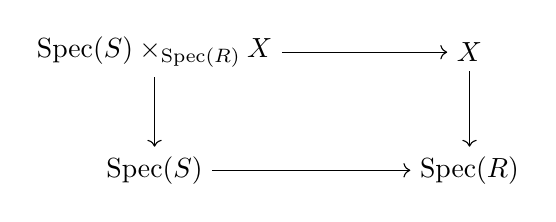
\begin{tikzpicture}
            \node (SX) at (0, 0) {$\Spec(S) \times_{\Spec(R)} X$};
            \node (S) at (0, -1.5) {$\Spec(S)$};
            \node (X) at (4, 0) {$X$};
            \node (R) at (4, -1.5) {$\Spec(R)$};

            \draw [->] (SX) -- (S);
            \draw [->] (SX) -- (X);
            \draw [->] (S) -- (R);
            \draw [->] (X) -- (R);
        \end{tikzpicture}
    \end{center}
    commute, is closed.
\end{lemma}
\begin{proof}
    Consider any scheme $Y$ over $\Spec(R)$.
    We have to show that the map $\pi: Y \times_{\Spec(R)} X \to Y$ that makes the diagram
    \begin{center}
        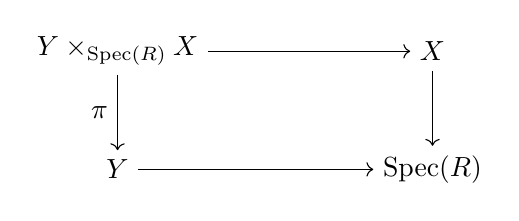
\begin{tikzpicture}
            \node (YX) at (0, 0) {$Y \times_{\Spec(R)} X$};
            \node (Y) at (0, -1.5) {$Y$};
            \node (X) at (4, 0) {$X$};
            \node (R) at (4, -1.5) {$\Spec(R)$};

            \draw [->] (YX) -- (Y) node [midway, left] {$\pi$};
            \draw [->] (YX) -- (X);
            \draw [->] (Y) -- (R);
            \draw [->] (X) -- (R);
        \end{tikzpicture}
    \end{center}
    commute, is closed.

    Let $Y = \bigcup_i V_i$ be a cover by affine opens.
    For each $i$, note that the diagram
    \begin{center}
        \begin{tikzpicture}
            \node (YX) at (0, 0) {$\pi^{-1}(V_i)$};
            \node (Y) at (0, -2) {$V_i$};
            \node (X) at (4, 0) {$X$};
            \node (R) at (4, -2) {$\Spec(R)$};

            \draw [->] (YX) -- (Y) node [midway, left] {$\pi_i := \restr{\pi}{\pi^{-1}(V_i)}$};
            \draw [->] (YX) -- (X);
            \draw [->] (Y) -- (R);
            \draw [->] (X) -- (R);
        \end{tikzpicture}
    \end{center}
    commutes.
    By the universal property of $V_i \times_{\Spec(R)} X$ we now find a morphism
    \begin{equation*}
        \psi: \pi^{-1}(V_i) \to V_i \times_{\Spec(R)} X
    \end{equation*}
    of schemes over $Y \times X$, i.e. the inclusion of $\pi^{-1}(V_i)$ into $Y \times_{\Spec(R)} X$ factors as
    \begin{equation*}
        \pi^{-1}(V_i) \ \overset{\psi}{\to} \ V_i \times_{\Spec(R)} X \ \to \ Y \times_{\Spec(R)} X
    \end{equation*}
    Considering $V_i \times_{\Spec(R)} X$ as an open subscheme of $Y \times_{\Spec(R)} X$, we thus see that $\psi$ must already be the identity and so $\pi^{-1}(V_i) \subseteq V_i \times_{\Spec(R)} X$.
    It follows that $\pi^{-1}(V_i) = V_i \times_{\Spec(R)} X$.
    By assumption, we now get that each $\pi_i$ is closed, as $V_i \cong \Spec(\O_Y(V_i))$ is affine.

    To show that $\pi$ is closed, let $C \subseteq Y \times_{\Spec(R)} X$ be closed.
    Consider some $x \in Y \setminus \pi(C)$.
    Since the $V_i$ cover $Y$, there is $i$ such that $x \in V_i$.
    As $\pi_i = \restr{\pi}{f^{-1}(V_i)}$ is closed, we see that
    \begin{equation*}
        \pi(C) \cap V_i = \pi_i(C \cap \pi^{-1}(V_i)) \quad \text{is closed in $V_i$}
    \end{equation*}
    Hence there is an open neighborhood $U \subseteq V_i$ of $x$ with $U \cap \pi(C) = \emptyset$.
    Now note that $V_i \subseteq Y$ is open, and so $U$ is also an open neighborhood of $x$ in $Y$.
    This holds for all $x \in Y \setminus \pi(C)$, hence $\pi(C)$ is closed.
\end{proof}
\begin{remark}
    \label{prop:functoriality_proj}
    Note that $\Proj$ is not functorial, in the sense that a homomorphism of graded rings $S \to T$ does not induce a natural morphism $\Proj(T) \to \Proj(S)$ (like $\Spec$ does).
    Namely, given $\alpha: S \to T$, we might want to consider
    \begin{equation*}
        \Proj(T) \to \Proj(S), \quad \p \mapsto \alpha^{-1}(\p)
    \end{equation*}
    However, in general this is not well-defined, as $\alpha^{-1}(\p)$ might contain $S_+$\footnote{Just consider the inclusion $R[x] \to R[x, y]$ and the ideal $\langle x \rangle \in \Proj(R[x, y])$.}.

    If we further require the map $\alpha: S \to T$ to fulfill $T_+ \subseteq \alpha(S_+)T$, then this works out and we get a morphism
    \begin{align*}
        \Proj(\alpha): \Proj(T) &\to \Proj(S), \quad \p \mapsto \alpha^{-1}(\p), \\
        \Proj(\alpha)^\#_{\D{f}}: \O_{\Proj(S)}(\D{f}) &\to \O_{\Proj(T)}(\D{\alpha(f)}), \quad \frac x y \mapsto \frac {\alpha(x)} {\alpha(y)}
    \end{align*}
    Note that this is indeed a well-defined morphism, as for $\p \in \Proj(T)$ there is some $f \in T_+ \setminus \p$ and by assumption, have $g \in S_+, t \in T$ with $\alpha(g)t = f$.
    Now $g \notin \alpha^{-1}(\p)$, as $g \in \alpha^{-1}(\p)$ would imply $\alpha(g) \in \p$, thus $f = t\alpha(g) \in \p$.

    In particular, any ring homomorphism $R \to S$ induces a canonical morphism $\P_S^n \to \P_R^n$ of schemes, since the induced ring homomorphism $R[x_0, ..., x_n] \to S[x_0, ..., x_n]$ satisfies the above additional condition.
\end{remark}
\begin{lemma}
    \label{prop:projective_space_base_change}
    Let $R \to S$ be a ring homomorphism.
    Then the base change of $\P_R^n$ is
    \begin{equation*}
        \P_R^n \times_{\Spec(R)} \Spec(S) \cong \P_S^n
    \end{equation*}
    as schemes over $\Spec(S)$.
\end{lemma}
\begin{proof}
    Consider the canonical map $\alpha: R[x_0, ..., x_n] \to S[x_0, ..., x_n]$ induced by $R \to S$.
    Note that
    \begin{equation*}
        S \otimes_R (R[x_0, ..., x_n]_f)_0 \cong (S[x_0, ..., x_n]_{\alpha(f)})_0 \quad \text{via} \quad \iota_f: s \otimes \frac r {f^n} \mapsto \frac {s\alpha(r)} {\alpha(f)^n}
    \end{equation*}
    for all homogeneous $f \in R[x_0, ..., x_n]$.
    By Lemma~\ref{prop:Df_affine}, we see that the basic open sets $\D{x_i}$ form an affine open cover of $\P_S^n$.
    Furthermore, we have a cover by affine opens $\D{x_i} \times_{\Spec(R)} \Spec(S)$ of $\P_R^n \times_{\Spec(R)} \Spec(S)$.
    Note that $\alpha(x_i) = x_i$.
    Together, we see that it suffices to show that the isomorphisms (induced by $\iota_{x_i}$)
    \begin{equation*}
        \phi_i: \D{x_i} = \Spec(S[x_0, ..., x_n]_{x_i})_0 \to \D{x_i} \times_{\Spec(R)} \Spec(S)
    \end{equation*}
    glue to an isomorphism $\Proj(S[x_0, ..., x_n]) \to \P_R^n \times_{\Spec(R)} \Spec(S)$.
    By the gluing lemma, it suffices that the compatibility conditions are satisfied, i.e. for all $i, j$ the diagram
    \begin{center}
        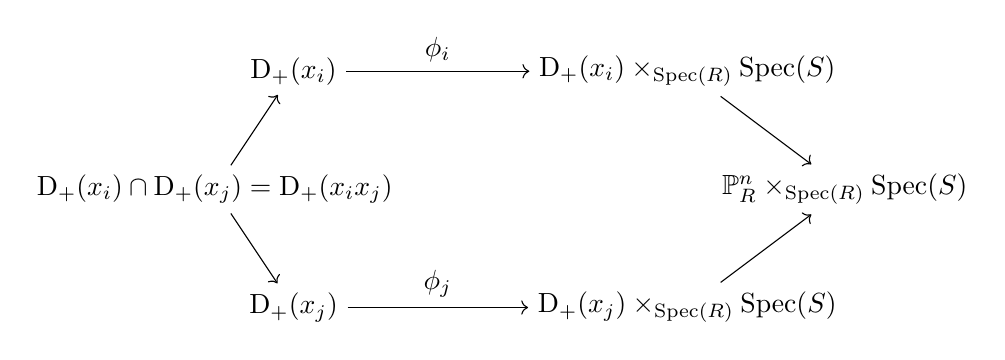
\begin{tikzpicture}
            \node (Sfg) at (1, 0) {$\D{x_i} \cap \D{x_j} = \D{x_ix_j}$};
            \node (Sf) at (2, 1.5) {$\D{x_i}$};
            \node (Sg) at (2, -1.5) {$\D{x_j}$};
            \node (f) at (7, 1.5) {$\D{x_i} \times_{\Spec(R)} \Spec(S)$};
            \node (g) at (7, -1.5) {$\D{x_j} \times_{\Spec(R)} \Spec(S)$};
            \node (all) at (9, 0) {$\P_R^n \times_{\Spec(R)} \Spec(S)$};

            \draw [->] (Sfg) -- (Sf);
            \draw [->] (Sfg) -- (Sg);
            \draw [->] (Sf) -- (f) node [midway, above] {$\phi_i$};
            \draw [->] (Sg) -- (g) node [midway, above] {$\phi_j$};
            \draw [->] (f) -- (all);
            \draw [->] (g) -- (all);
        \end{tikzpicture}
    \end{center}
    commutes.

    For a prime ideal $\p \in \D{x_ix_j}$ have that
    \begin{equation*}
        \phi_i(\p) = \iota_{x_i}^{-1}\bigl( \p \cap (S[x_0, ..., x_n]_{x_i})_0 \bigr) \in \D{x_i} \times_{\Spec(R)} \Spec(S)
    \end{equation*}
    and so $x_j \notin \phi_i(\p)$, i.e. $\phi_i(\p) \in \D{x_ix_j} \times_{\Spec(R)} \Spec(S)$.
    Hence, both restrictions
    \begin{equation*}
        \restr{\phi_i}{\D{x_ix_j}}, \ \restr{\phi_j}{\D{x_ix_j}}: \D{x_ix_j} \to \D{x_ix_j} \times_{\Spec(R)} \Spec(S)
    \end{equation*}
    map into $\D{x_ix_j} \times_{\Spec(R)} \Spec(S)$.
    Now note that the diagram
    \begin{center}
        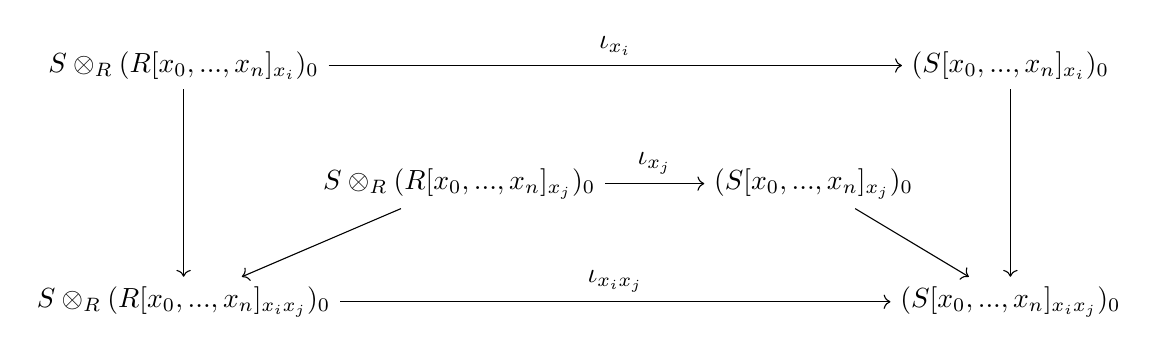
\begin{tikzpicture}
            \node (Rf) at (-3, 0) {$S \otimes_R (R[x_0, ..., x_n]_{x_i})_0$};
            \node (Rg) at (0.5, -1.5) {$S \otimes_R (R[x_0, ..., x_n]_{x_j})_0$};
            \node (Rfg) at (-3, -3) {$S \otimes_R (R[x_0, ..., x_n]_{x_ix_j})_0$};

            \node (Sf) at (7.5, 0) {$(S[x_0, ..., x_n]_{x_i})_0$};
            \node (Sg) at (5, -1.5) {$(S[x_0, ..., x_n]_{x_j})_0$};
            \node (Sfg) at (7.5, -3) {$(S[x_0, ..., x_n]_{x_ix_j})_0$};

            \draw [->] (Rf) -- (Sf) node [midway, above] {$\iota_{x_i}$};
            \draw [->] (Rg) -- (Sg) node [midway, above] {$\iota_{x_j}$};
            \draw [->] (Rfg) -- (Sfg) node [midway, above] {$\iota_{x_ix_j}$};

            \draw [->] (Rf) -- (Rfg);
            \draw [->] (Rg) -- (Rfg);
            \draw [->] (Sf) -- (Sfg);
            \draw [->] (Sg) -- (Sfg);
        \end{tikzpicture}
    \end{center}
    commutes, and so the restrictions of $\phi_i$ resp. $\phi_j$ to $\D{x_ix_j}$ are both induced by the homomorphism $\iota_{x_ix_j}$, hence they are equal.
    The claim follows.
\end{proof}
This lemma also justifies the usual definition of projective $n$-space over a scheme $B$ as
\begin{equation*}
    \P_B^n := B \times_{\Spec(\Z)} \P_\Z^n
\end{equation*}

Before we come to the proof of properness now, there is one last notion to present.
\begin{definition}
    Let $x \in X$ be a point in a scheme (or more generally, a topological space).
    A point $x' \in X$ is said to \emph{specialize} $x$, if it is contained in the closure $x' \in \overline{\{x\}}$.
\end{definition}
The next lemma is directly from \cite[II.4.5]{hartshorne}.
\begin{lemma}
    \label{prop:im_closed_iff_stable_specialization}
    Let $f: X \to Y$ be a quasi-compact morphism.
    Then $f(X)$ is closed if and only if it is stable under specialization.
\end{lemma}
\begin{proof}
    The implication $\Leftarrow$ is clear.
    It suffices to show that $f(X) \cap V \subseteq V$ is closed for all affine opens $V \subseteq Y$.
    
    Note that the preimage $f^{-1}(V)$ is quasi-compact, hence has a finite cover of affine opens $U_i \subseteq X$.
    Now let $V_i = \overline{f(U_i)}$ be the closed subscheme of $V$ with the canonical (reduced) scheme structure\footnote{As in the Lecture Notes, Section 5.6.}.
    Since $V$ is affine, also $V_i$ is affine.
    Note that now it suffices to show that $f(U_i) \subseteq V_i$ is closed.

    In other words, we have reduced the situation to the case that
    \begin{equation*}
        f' = \restr{f}{U_i}: U_i = \Spec(A) \to V_i = \Spec(B)
    \end{equation*}
    is a morphism between affine schemes with dense image.
    We want to show that $f'(U_i)$ is already $V_i$, i.e. $V_i \subseteq f(U_i)$.

    Consider some $\p \in V_i$.
    By Zorn's Lemma, there is a minimal prime ideal $\p' \subseteq \p$ in the ring $B$.
    Note that $\p$ is a specialization of $\p'$.
    Hence, it suffices to show that $\p' \in f'(U_i)$.
    Note that $B_{\p'}$ must be a field, otherwise we could take a proper nonzero prime ideal of $B_{\p'}$ and its preimage under $B \to B_{\p'}$ would be a smaller prime ideal in $B$.

    Since $f': \Spec(A) \to \Spec(B)$ has dense image, we find that $B \to A$ is injective.
    Consider $A$ as a $B$-algebra.
    Let $\q$ be a prime ideal of $A \otimes_B B_{\p'}$ (this is not the zero ring, as $B_{\p'}$ is a flat $B$-module and so the inclusion $B \to B_{\p'}$ induces an inclusion $B_{\p'} \to A \otimes_B B_{\p'}$).

    Taking the preimage of $\q$ under the map $A \to A \otimes_B B_{\p'}$ now gives a prime ideal $\q' \leq A$.
    Since $\q \cap B_{\p'} = \{ 0 \}$ (here we use that $B_{\p'}$ is a field), find $\q' \cap B = \p'$, thus $\q'$ maps to $\p'$ under $\Spec(A) \to \Spec(B)$.
    This shows $\p' \in f'(U_i)$ and the claim follows.
\end{proof}
The next lemma is now the decisive statement that will allow us to show that $\P_R^n \to \Spec(R)$ is closed.
It is also the place where things get somewhat ugly, and we require a good deal of commutative algebra to prove it.
\begin{lemma}
    \label{prop:adding_coeff_ideal_does_not_introduce_irrelevant_ideal}
    Let $\p \in \Proj(R[x_0, ..., x_n])$ and let $\q \leq R$ be a prime ideal such that $\p \cap R \subseteq \q$.
    Then there some $i$ such that no $\alpha x_i^m$ is in $\b := \p + \q R[x_0, ..., x_n]$, for any $\alpha \in R \setminus \b$ and any $m \in \N$.
\end{lemma}
\begin{proof}
    Assume for a contradiction  that there is $m \in \N$ such that $\alpha_i x_i^m \in \b$ for all $i$ and some $\alpha_i \in \b \setminus R$.
    Since $\b \cap R = \q$ is prime, have that $\alpha := \prod_i \alpha_i \notin \b$ and further $\alpha^n \notin \b$ for all $n \in \N$.
    Furthermore, we obviously have $\alpha x_i^m \in \b$ for all $i$.

    Consider now the vector $(w_i)_{i < N}$ containing all monomials of degree $(n + 1)m$.
    By assumption, all\footnote{Since a monomial of degree $(n + 1)m$ in $n + 1$ variables is divisible by $x_i^m$ for at least one $i$, by the pigeonhole principle.} $\alpha w_i \in \b$.
    Since $\p$ is homogeneous, observe that by definition of $\b$, there are $r_{ij} \in \q$ such that
    \begin{equation*}
        \alpha w_i - \sum_{j < N} r_{ij} w_j \in \p
    \end{equation*}
    Working modulo $\p$, we see that $A w = \alpha w$ where $A \in (\b/\p)^{N \times N}$ is a matrix with coefficients in $\b/\p$.

    Now observe that no power of $\alpha$ is in $\b/\p$ (as mentioned before).
    Hence there exists a prime ideal\footnote{By the usual argument, i.e. take a preimage of a prime ideal under the map $R \to R/\p \to (R/\p)_\alpha$.} in $R/\p$ containing $\b/\p$ and not containing $\alpha$.
    Localizing at that prime ideal gives a local ring $S$ with maximal ideal $\mathfrak{l}$.
    Now we continue in $S$, replacing $w$ and $A/\alpha$ by their images under $R \to S$.
    So $w \in S^N$ and $A/\alpha \in \mathfrak{l}^{N \times N}$.
    Note that we still have $(A/\alpha) w = w$.

    wlog $S$ is Noetherian, otherwise continue with the ring
    \begin{equation*}
        \tilde{S} := \bigl( \Z / \mathrm{char}(S) \Z \bigr) \bigl[ A/\alpha, x \bigr]
    \end{equation*}
    generated by the coefficients of $A/\alpha$ and $w$ (this is Noetherian, as it is a quotient of a polynomial ring in finitely many variables).
    
    Now equip $S$ with the $\mathfrak{l}$-adic topology.
    Note that $S$ is Noetherian and local, thus the Krull intersection theorem \cite[8.41]{comalg_notes} shows that the $\mathfrak{l}$-adic topology is Hausdorff and we find
    \begin{equation*}
        w = \lim_{i \to \infty} w = \lim_{i \to \infty} \frac {A^i} {\alpha^i} w = \Bigl( \lim_{i \to \infty} \frac {A^i} {\alpha^i} \Bigr) w = 0 w = 0
    \end{equation*}
    since $(A/\alpha)^i$ has coefficients in $\mathfrak{l}^i$, thus converges to $0$ as $i \to \infty$.

    Thus $w \equiv 0 \mod \p$ and so $x_i^N \equiv 0 \mod \p$, i.e. $x_i^N \in \p$ for all $i$.
    However, since $\p$ is prime, this implies $R[x_0, ..., x_n]_+ = \langle x_0, ..., x_n \rangle \subseteq \p$, contradicting the assumption. 
\end{proof}
As we will see in the next proof, this lemma shows that if $\P_R^n \to \Spec(R)$ maps a point $\p$ to a point $\q$, then it also maps a specialization of $\p$ to any specialization of $\q$.
From this, we can derive the next proposition.
\begin{prop}
    \label{prop:projective_structure_morphism_closed}
    The morphism $\P_R^n \to \Spec(R)$ is closed.
\end{prop}
\begin{proof}
    Denote $\P_R^n \to \Spec(R)$ by $\phi$.
    Consider a closed set $\V{\a} := \P_R^n \setminus \D{\a}$ given by a homogeneous ideal $\a \leq R[x_0, ..., x_n]$.
    By Lemma~\ref{prop:im_closed_iff_stable_specialization}, it suffices to show that $\phi(\V{\a})$ is closed under specialization (note that $\P_R^n \to \Spec(R)$ is quasi-compact, e.g. by Proposition~\ref{prop:p_quasi_compact}).

    Consider $\q \in \phi(\V{\a}) \subseteq \Spec(R)$ and a prime ideal $\q'$ that specializes $\q$, i.e. $\q' \supseteq \q$.
    Then there is a $\p \in \V{\a}$ with $\p \cap R = \q$, in particular $\a \subseteq \p$.
    We want to show that $\q' \in \phi(\V{\a})$.

    Note that by Lemma~\ref{prop:adding_coeff_ideal_does_not_introduce_irrelevant_ideal}, there is $i$ such that the multiplicative set
    \begin{equation*}
        T := \{ \alpha x_i^m \ | \ \alpha \in R \setminus \q', \ m \in \N \}
    \end{equation*}
    has empty intersection with the ideal $\b := \p + \q' R[x_0, ..., x_n]$.
    
    Hence, the ring $T^{-1}(R[x_0, ..., x_n]/\b)$ is nonzero, thus has a prime ideal.
    Taking its preimage under
    \begin{equation*}
        R[x_0, ..., x_n] \to R[x_0, ..., x_n]/\b \to T^{-1}(R[x_0, ..., x_n]/\b)
    \end{equation*}
    yields a prime ideal $\p'$ such that $x_i \notin \p'$ and $\b \subseteq \p'$.
    Clearly have that $\q' \subseteq \p'$ and since $\p' \cap T = \emptyset$, find that $\p' \cap R = \q'$.
    By Lemma~\ref{prop:homogeneous_part_prime}, assume wlog that $\p'$ is homogeneous.
    Now have a homogeneous prime ideal $\p'$ with $\a \subseteq \p \subseteq \p'$, i.e. $\p' \in \V{\a}$ and $\phi(\p') = \p' \cap R = \q'$.
    Thus $\q \in \phi(\V{\a})$ and the claim follows.
\end{proof}
I must say, I find this proof and also the more geometric proof later (Proposition~\ref{prop:projective_space_proper_alternative_proof}) extremely fascinating.
In particular, I like how generic points are quite important for the proof.
It also reminds me of the only classical proof of an equivalent statement (projections from projective space are closed) I have ever seen.
The idea was - more or less - to consider points $y \in \im(f) \subseteq \P_k^n$ with preimages $x \in X \subseteq \P_k^m$ and deduce (using Hilbert's Nullstellensatz) that there is some ``generic preimage'' $\tilde{x} \in \P_K^m$ in projective space over the algebraic closure $K = \overline{k(Y)}$ of the ``generic point'' $\tilde{y} = [y_0 : ... : y_n] \in \P_K^n$.
A ``partial evaluation homomorphism'' (i.e. not defined on the whole domain) $K \dashrightarrow k$ can then be used to ``evaluate'' the ``generic preimage point'' on each image point.
The core of that proof is exactly constructing this ``partial evaluation homomorphism'', which corresponds exactly to Lemma~\ref{prop:adding_coeff_ideal_does_not_introduce_irrelevant_ideal}.

But now enough of talking, here is the main corollary, which is also the main result of the miniproject.
\begin{corollary}
    The morphism $\P_R^n \to \Spec(R)$ is universally closed.
\end{corollary}
\begin{proof}
    Use Lemma~\ref{prop:universally_closed_affines}, so consider an affine base change $f_{\Spec(S)}: \P_R^n \times_{\Spec(R)} \Spec(S) \to \Spec(S)$.
    By Lemma~\ref{prop:projective_space_base_change}, have that $\P_R^n \times_{\Spec(R)} \Spec(S) \cong \P_S^n$ as schemes over $S$, hence $f_{\Spec(S)}$ is isomorphic to $\P_S^n \to \Spec(S)$.
    This morphism is closed by Proposition~\ref{prop:projective_structure_morphism_closed} and the claim follows.
\end{proof}
\begin{corollary}
    Projective space $\P_R^n$ over $\Spec(R)$ is proper.
\end{corollary}
\begin{corollary}
    Let $k$ be an algebraically closed field.
    Then projective space $\P_k^n$ over $\Spec(k)$ is a complete variety.
\end{corollary}

\section{Valuative criterion of properness}
\label{sec:valuative_criterion_properness}
Instead of using some magical ad-hoc argument as before, there is also the following nice characterization of the notion of properness.
We will omit the proof here, but present the statement as it can give more geometric intuition on properness and why $\P_R^n$ is proper.
\begin{prop}
    \label{prop:valuative_criterion_properness}
    Let $X$ be Noetherian and $f: X \to Y$ a morphism of finite type.
    The following are equivalent
    \begin{itemize}
        \item $f$ is proper
        \item For every valuation ring $R$ with field of fractions $K = \Frac(R)$ and all morphisms $\Spec(R) \to Y$, $\Spec(K) \to X$ that make the diagram
        \begin{center}
            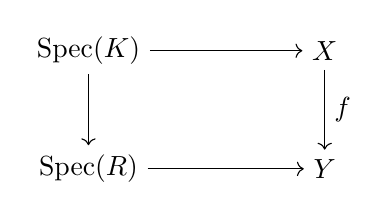
\begin{tikzpicture}
                \node (K) at (0, 0) {$\Spec(K)$};
                \node (R) at (0, -1.5) {$\Spec(R)$};
                \node (X) at (3, 0) {$X$};
                \node (Y) at (3, -1.5) {$Y$};
    
                \draw [->] (K) -- (R);
                \draw [->] (K) -- (X);
                \draw [->] (R) -- (Y);
                \draw [->] (X) -- (Y) node [midway, right] {$f$};
            \end{tikzpicture}
        \end{center}
        commute, there exists a unique compatible morphism $\Spec(R) \to X$.
    \end{itemize}
\end{prop}
\begin{proof}
    Omitted, see e.g. \cite[II.4.7]{hartshorne} or \citestacks{0BX5}.
\end{proof}
\begin{prop}
    \label{prop:projective_space_proper_alternative_proof}
    The morphism $\P_R^n \to \Spec(R)$ is proper.
\end{prop}
\begin{proof}[Alternative Proof]
    Since properness is preserved under base change, by Lemma~\ref{prop:projective_space_base_change} it suffices to show the statement for $\P_\Z^n \to \Spec(\Z)$.

    Apply Proposition~\ref{prop:valuative_criterion_properness}.
    Let $R$ be a valuation ring, $K = \Frac(R)$ and assume we have morphisms $\Spec(R) \to Y$, $\Spec(K) \to X$ such that the diagram
    \begin{center}
        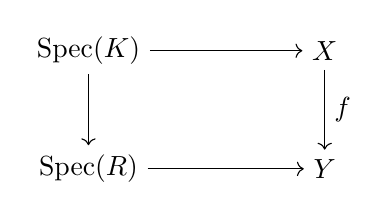
\begin{tikzpicture}
            \node (K) at (0, 0) {$\Spec(K)$};
            \node (R) at (0, -1.5) {$\Spec(R)$};
            \node (X) at (3, 0) {$X$};
            \node (Y) at (3, -1.5) {$Y$};

            \draw [->] (K) -- (R);
            \draw [->] (K) -- (X);
            \draw [->] (R) -- (Y);
            \draw [->] (X) -- (Y) node [midway, right] {$f$};
        \end{tikzpicture}
    \end{center}
    commutes.
    Note that $\Spec(K) = \{ \langle 0 \rangle \}$, so let $\xi \in X$ be the image of $\langle 0 \rangle$ under $\Spec(K) \to X$.
    Since $\langle x_0, ..., x_n \rangle \not\subseteq \xi$, there is $x_i \not\in \xi$.
    Now let
    \begin{equation*}
        f_j := \begin{cases}
            x_j & \text{if $x_j \notin \xi_1$} \\
            x_j - x_i & \text{if $x_j \in \xi_1$}
        \end{cases}
    \end{equation*}
    Thus all $f_j$ are homogeneous of degree 1 with $\langle f_j \ | \ j \rangle = \langle x_0, ..., x_n \rangle$.
    It follows that $X = \bigcup_j \D{f_j}$ is a cover by affine opens such that $\xi \in \bigcap_j \D{f_j}$.
    Now possibly apply a linear automorphism $f_j \to x_j$, so have wlog $f_j = x_j$.
    In particular, find $x_j \in \O_{X, \xi_1}^*$.

    The morphism $\Spec(K) \to X$ now gives an inclusion $k(\xi) \subseteq K$.
    Since $x_j \in \O_{X, \xi}^*$, observe that $g_{ij} := x_i / x_j \in K$ is well-defined and nonzero with $g_{ij} g_{jk} = g_{ik}$.

    As $R$ is a valuation ring, we find $k$ such that $g_{k0}$ is the smallest element (w.r.t. divisibility by $R$) among $g_{00}, ..., g_{n0}$.
    So we see that $g_{jk} = g_{j0} / g_{k0} \in R$ for all $i$.
    In particular, we find a ring homomorphism
    \begin{equation*}
        \Z\left[ \frac {x_0} {x_k}, ..., \frac {x_n} {x_k} \right] \to R, \quad \frac {x_j} {x_k} \mapsto g_{i k}
    \end{equation*}
    that is compatible with the field inclusion $k(\xi) \subseteq K$.

    The induced morphism
    \begin{equation*}
        \Spec(R) \to \Spec(\Z\Bigl[ \frac {x_0} {x_k}, ..., \frac {x_n} {x_k} \Bigr]) = \D{x_k} \subseteq X
    \end{equation*}
    is now a compatible morphism $\Spec(R) \to X$.
    
    It is not hard to show that the morphism is unique\footnote{In fact, the statement that there is at most one such morphism is equivalent to $\P_R^n \to \Spec(R)$ being separated (by \citestacks{01L0}), so follows from Proposition~\ref{prop:projective_space_separated}.}, and the claim follows.
\end{proof}
Note that in some way, this is the same proof as before.
The core idea - namely the choice of the smallest element $g_{k0}$ (w.r.t. divisibility by $R$) - more or less achieves the same effect as the more complicated ideal argument from Lemma~\ref{prop:adding_coeff_ideal_does_not_introduce_irrelevant_ideal}.
\printbibliography
\end{document}